\documentclass[tikz,border=5pt]{standalone}
\usetikzlibrary{positioning,arrows.meta}

\begin{document}

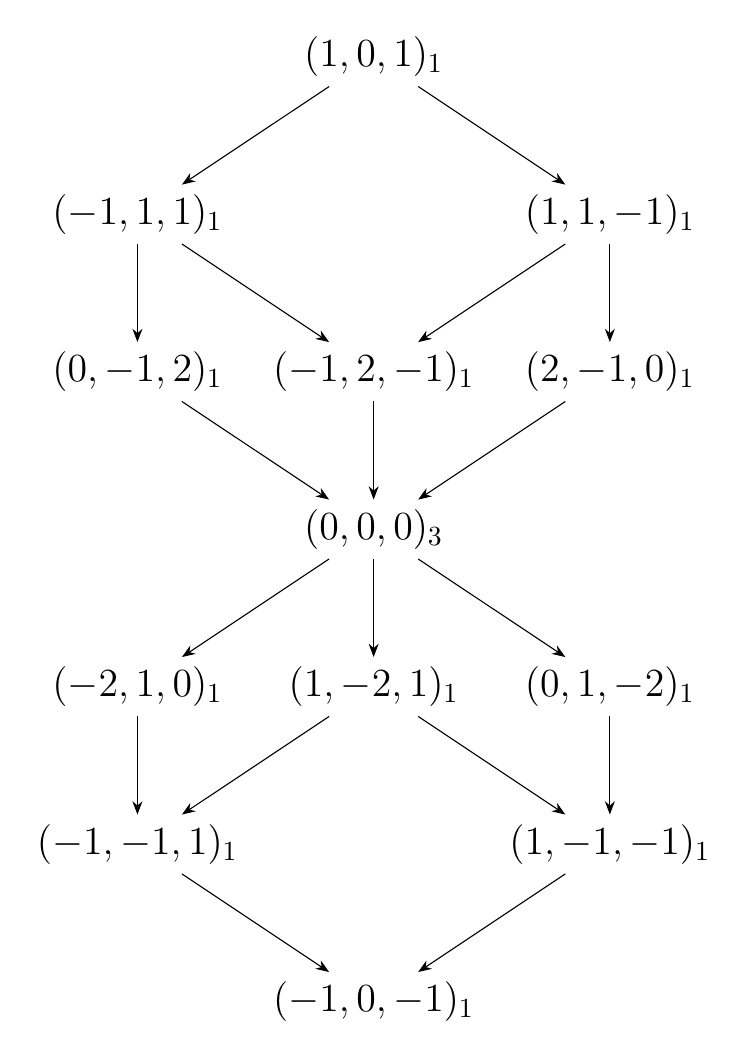
\begin{tikzpicture}[
    >=Stealth,
    every node/.style={font=\Large},
    node distance=2.3cm
]

\node (a) at (3,0) {$(1, 0, 1)_1$};

\node (b1) at (0,-2.0) {$(-1, 1, 1)_1$};
\node (b2) at (6,-2.0) {$(1, 1, -1)_1$};

\node (c1) at (0,-4.0) {$(0, -1, 2)_1$};
\node (c2) at (3,-4.0) {$(-1, 2, -1)_1$};
\node (c3) at (6,-4.0) {$(2, -1, 0)_1$};

\node (d) at (3,-6.0) {$(0, 0, 0)_3$};

\node (e1) at (0,-8.0) {$(-2, 1, 0)_1$};
\node (e2) at (3,-8.0) {$(1, -2, 1)_1$};
\node (e3) at (6,-8.0) {$(0, 1, -2)_1$};

\node (f1) at (0,-10.0) {$(-1, -1, 1)_1$};
\node (f2) at (6,-10.0) {$(1, -1, -1)_1$};

\node (g) at (3,-12.0) {$(-1, 0, -1)_1$};

\draw[->] (a) -- (b1);
\draw[->] (a) -- (b2);

\draw[->] (b1) -- (c1);
\draw[->] (b1) -- (c2);
\draw[->] (b2) -- (c2);
\draw[->] (b2) -- (c3);

\draw[->] (c1) -- (d);
\draw[->] (c2) -- (d);
\draw[->] (c3) -- (d);

\draw[->] (d) -- (e1);
\draw[->] (d) -- (e2);
\draw[->] (d) -- (e3);

\draw[->] (e1) -- (f1);
\draw[->] (e2) -- (f1);
\draw[->] (e2) -- (f2);
\draw[->] (e3) -- (f2);

\draw[->] (f1) -- (g);
\draw[->] (f2) -- (g);

\end{tikzpicture}

\end{document}